\documentclass[coverpage]{article}
\usepackage[margin=1in]{geometry}
\usepackage{pdfpages}
\usepackage{wrapfig}
\usepackage{amsmath}

\newcommand{\loggerpro}{\textit{Logger Pro}\texttrademark}
\newcommand{\origin}{\textit{Origin Pro}\texttrademark}

\title{Rotational Kinetic Energy Lab}
\date{October 31, 2023}
\author{Wolf S. Mermelstein}

\begin{document}
	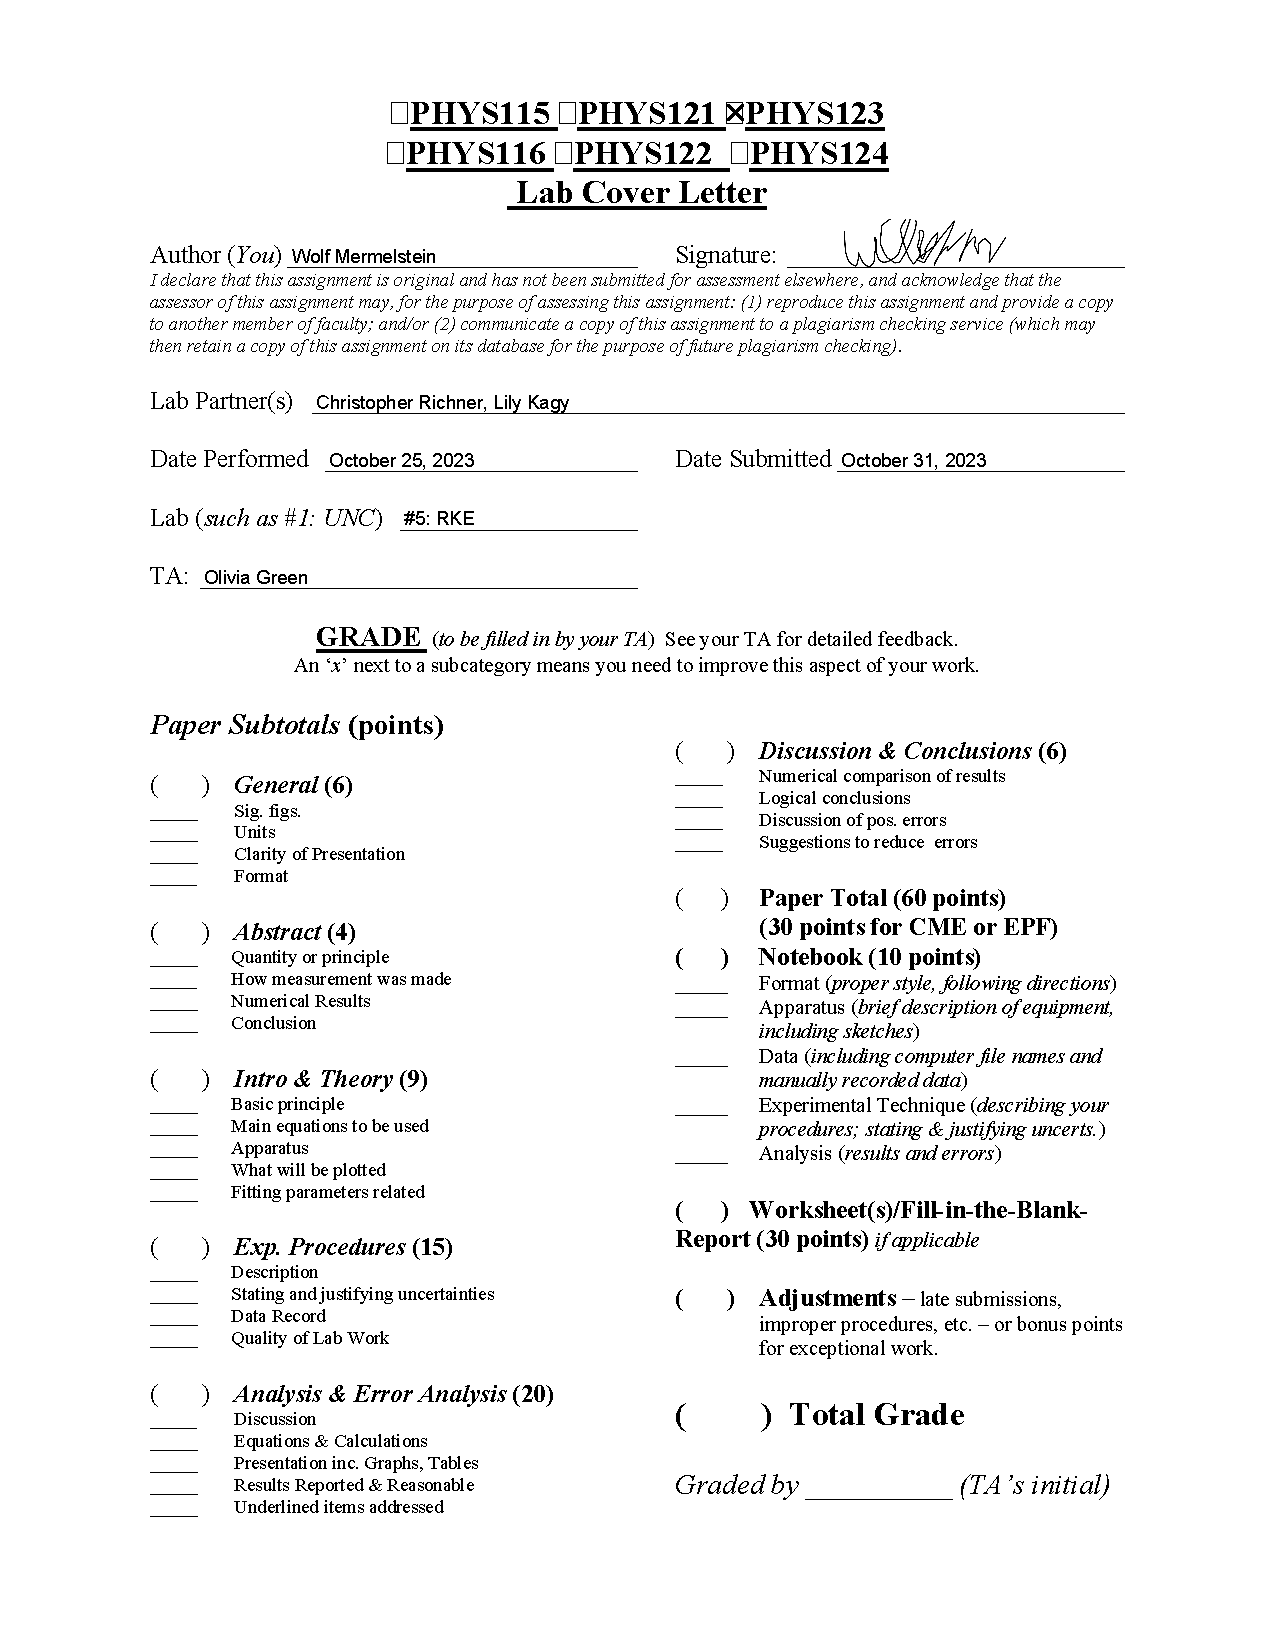
\includepdf{reportCover.pdf}
	
	\maketitle
	
	\begin{abstract}
		content...
	\end{abstract}
	
	\tableofcontents
	
	\twocolumn
	
	\section{Introduction}
	
	\subsection{Moment of Inertia}
	
	Moment of inertia, often denoted by $I$, is a function of the specific geometry and mass distribution of an object. Moment of inertia is implicitly relative to the axis of rotation. Where $R$ is the distance from the axis of rotation and $M$ is the mass of the object, for a point mass the moment of inertia, $I$, is given by
	
	\begin{align}
		I=MR^2
	\end{align}

	The entire moment of inertia can be computed by thinking of a given object as a collection of tiny masses. As the masses' volumes shrink down to some small volume with some proportionately small mass, the can then be eventually said to be the differential $dM$. Integrating all the small point masses across the entire object implies that the entire moment of inertia of an object, $I_{tot}$, is given by
	
	\begin{align}
		I=\sum_{k=1}^{\infty}{\frac{m}{k}R^2}\\
		=\int{R^2dM}
	\end{align}

	This is conceptually helpful in understanding moment of inertia for arbitrary shapes, but is not practically useful for non simple (i.e. circles, squares, collections of discreet point masses) shapes, such as the mass-loaded, spoked wheel that we used in our experiment. As a result of such, it is often helpful to actually measure moment of inertia instead of attempting to compute it.
	
	\subsection{Conservation of Energy}
	
	The translational kinetic energy of an object in motion with mass $M$ moving at speed $v$ is given to be
	
	\begin{align}
		K_T&=\frac{1}{2}Mv^2 \label{eq:translational-kinetic}
	\end{align}

	Since we know that
	
	\begin{align}
		\frac{\theta}{2\pi} = \frac{s}{2\pi R} \notag \\
		s=\theta R
	\end{align}

	and 
	
	\begin{align}
		\frac{d}{dt}s = \frac{d}{dt}\theta R \notag \\
		v = \omega r \label{eq:omega-v-relationship}
	\end{align}

	We can then derive from equation \ref{eq:translational-kinetic} that the rotational kinetic energy, $K_R$, is
	
	\begin{align}
		K_R = \frac{1}{2}M(\omega R)^2 \notag \\
		= \frac{1}{2} (M R^2) \omega^2 \notag \\
		= \frac{1}{2} I \omega^2 \label{eq:rotational-kinetic}
	\end{align}

	where $I$ is defined to be the moment of inertia about the axis of rotation.
	
	For the mass in figure \ref{fig:apparatus}~descends downwards due to gravity, it begins to lose its gravitational potential energy, $U_W$. The total energy of the system is internally conserved, however a small amount of energy is lost due to friction. So, where $\Delta{U}_W$ is the change in the gravitational potential energy of the counterweight, $K_T$ is the translational kinetic energy of the counterweight, and $K_R$ is the rotational kinetic energy of the counterweight, we state that
	
	\begin{align}
		\Delta{U}_W + K_T + K_R = W_f
	\end{align}

	Which, using equations \ref{eq:rotational-kinetic} and \ref{eq:translational-kinetic}, implies that
	
	\begin{align}
		\Delta{U}_W + (\frac{1}{2} M v^2) + (\frac{1}{2} I \omega^2) = W_f
	\end{align}

	$\Delta{U}_W$ should be negative, and $K_T$ \& $K_R$ positive because the mass is falling, and, thus, losing gravitational kinetic energy, whilst simultaneously proportionately gaining kinetic energy.
	
	Using the fact that gravitational potential energy for an object at height $h$ of mass $m$ in an environment where gravity can be approximated to $g$ is given to be
	
	\begin{align}
		U_G = (M \cdot g \cdot h)
	\end{align}
	
	Plugging this in, and renaming $h$ be $y$, we get the final equation
	
	\newcommand{\mgy}{(M \cdot g \cdot y)}
	
	\begin{align}
		-\mgy + (\frac{1}{2} M v^2) + (\frac{1}{2} I \omega^2) = W_f \label{eq:total-energy-with-friction}
	\end{align}
	
	\subsection{Working Equation}
	
	Since for our specific experiment we used paperclips attached to the counterweight to cancel out friction, we can instead rewrite equation \ref{eq:total-energy-with-friction} to be
	
	\begin{align}
		-\mgy + (\frac{1}{2} M v^2) + (\frac{1}{2} I \omega^2) = 0
	\end{align}
	
	Carefully noting that we have discluded the energy of the moving paperclips, as it is negligible in comparison to the other energies of the system. And, to further simplify things, we will define $y$ to be vertically positive, so as to make the equation into
	
	\begin{align}
		-\mgy + (\frac{1}{2} M v^2) + (\frac{1}{2} I \omega^2) = 0
	\end{align}

	Then, using relationship \ref{eq:omega-v-relationship}, we plug in $\frac{v}{r}$ for $\omega$, resulting in the equation
	
	\begin{align}
		-\mgy + (\frac{1}{2} M v^2) + (\frac{1}{2} I (\frac{v}{r})^2) = 0 \notag \\
		= \frac{1}{2} \cdot v^2 \cdot (M + \frac{I}{r^2})
	\end{align}

	Or, as will be used more frequently for our computations, the equivalent equation in the form
	
	\begin{align}
		gy = \frac{1}{2}(1 + \frac{I}{Mr^2}) \cdot v^2
	\end{align}
	
	\section{Procedure}
	
	\begin{figure}
		\centering
		\caption{Visual representation of $k$ and $r$}
		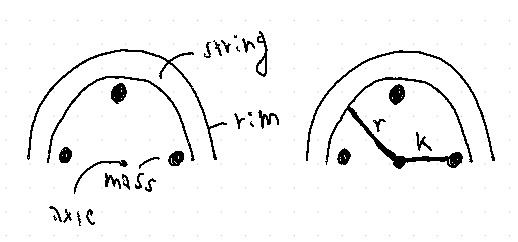
\includegraphics[width=2.3in]{graphics/rAndK.png}
	\end{figure}

	\begin{figure}
		\label{fig:apparatus}
		\caption{Roto-Dyne Inertia Wheel Apparatus \cite{labManual}}
		\centering
		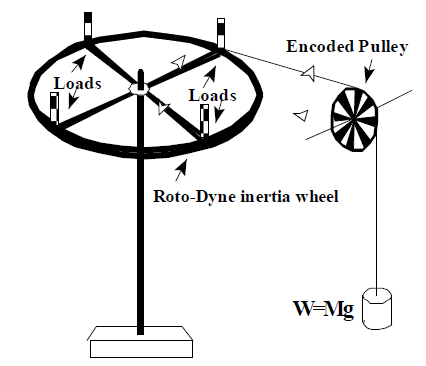
\includegraphics[width=2in]{graphics/apparatus.png}
	\end{figure}
	
	Before conducting our experiment, we took measurements of various parts of our setup. First we obtained $d$ from the lab manual, twice the distance from the axle of the wheel to the string, and then we measured $k$, the distance from the axle of the wheel to the masses. We determined $r$ to be half the diameter. For $r$ we used the provided uncertainty of $\pm 0.002 \text{m}$, whereas for $k$ we measured very carefully and chose the uncertainty to be $0.001 \text{m}$
	
	\begin{align}
		d&=0.200 \pm 0.002\ \text{m} \notag \\
		r&= 0.100 \pm 0.002\ \text{m} \notag \\
		k&=0.073 \pm 0.001\ \text{m} \notag
	\end{align}

	We used a counterweight with a given mass of $0.06\text{kg}$ to provide a torque to spin our Roto-Dyne wheel, as can be seen in figure~\ref{fig:apparatus}. To account for friction, we incrementally added paperclips to the bottom of the counterweight. We continued to add paperclips up until the mass would fall at a constant speed to counteract the force of friction, using \loggerpro~software and an encoded pulley to monitor acceleration and velocity. Let $M_c$ be the mass of the counterweight and $M_p$ be the mass of the paperclips opposing friction, not used in our computations but still important to the experimental design.
	
	\begin{align}
		M_p&=0.0015 \pm 0.0001\ \text{kg} \notag \\
		M_c&=0.06\ \text{kg} \notag
	\end{align}

	Also, we were provided with the mass of the Roto-Dyne wheel, $M_R$ and the mass loads, $M_L$.
	
	\begin{align}
		M_R&=1.5\ \text{kg} \notag \\
		M_L&=.225 \pm .002\ \text{kg} \notag
	\end{align}
	
	For the encoded pulley that we used to measure velocity and length of unrolled string it was given that the gaps between intervals of measurement, $\Delta{s}$, was
	
	\begin{align}
		\Delta{s}=0.015\ \text{m} \notag
	\end{align}
	
	\section{Results}
	
	\section{Analysis}
	
	\section{Conclusion}
	
	\section*{Acknowledgments}
	I would like to thank Christopher Richner and Lily Kagy, CWRU Department of Physics, for their help in obtaining the experimental data, collaborating on preparation of the figures, and checking calculations. Additionally, I would like to thank Olivia Green, CWRU Department of Physics, for helping facilitate our lab.
	
	\bibliographystyle{plain}
	\nocite{textbook}
	\nocite{labManual}
	\bibliography{sources}
\end{document}